% Intentar replicar este dibujo https://xkcd.com/1022/
% No seais duros que es mi primer dibujo con tikz :-(

\documentclass[tikz]{standalone}

\begin{document}

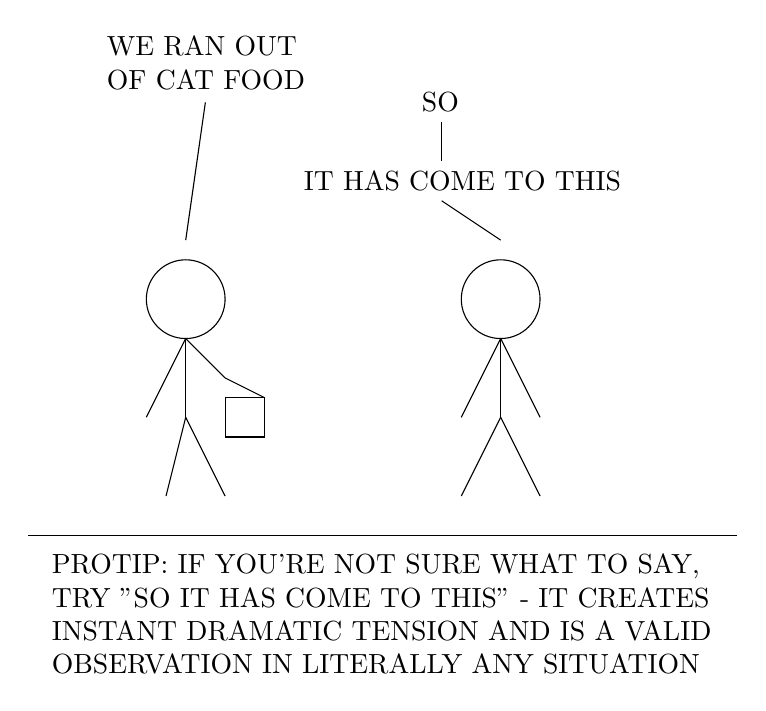
\begin{tikzpicture}
%\draw[help lines](0,0) grid (9,9);
\draw[-] (0,2) -- (9,2); % suelo

\draw (6.0,5.0) circle (0.5); % cabeza 2
\draw (2.0,5.0) circle (0.5); % cabeza 1

\draw[-] (2,3.5) -- (2.0,4.5); % cuerpo 1
\draw[-] (6,3.5) -- (6.0,4.5); % cuerpo 2

\draw[-] (1.5,3.5) -- (2.0,4.5); % brazo 1.1
\draw[-] (2.5,4.0) -- (2.0,4.5); % brazo 1.2.1
\draw[-] (3.0,3.75) -- (2.5,4.0); % brazo 1.2.2
\draw[-] (1.75,2.5) -- (2.0,3.5); % pierna 1.1
\draw[-] (2.5,2.5) -- (2.0,3.5); % pierna 1.2

\draw[-] (5.5,3.5) -- (6.0,4.5); % brazo 2.1
\draw[-] (6.5,3.5) -- (6.0,4.5); % brazo 2.2
\draw[-] (5.5,2.5) -- (6.0,3.5); % pierna 2.1
\draw[-] (6.5,2.5) -- (6.0,3.5); % pierna 2.2

\draw (2.5,3.25) rectangle (3.0,3.75); % bolsa

\node[text width=3cm] at (2.5,8.0) {WE RAN OUT OF CAT FOOD}; % texto 1
\node[text width=2cm] at (6.0,7.5) {SO}; % texto 2.1
\node[text width=5cm] at (6.0,6.5) {IT HAS COME TO THIS}; % texto 2.2
\node[text width=8.4cm] at (4.5,1.0) {PROTIP: IF YOU'RE NOT SURE WHAT TO SAY, TRY "SO IT HAS COME TO THIS" - IT CREATES INSTANT DRAMATIC TENSION AND IS A VALID OBSERVATION IN LITERALLY ANY SITUATION}; % texto suelo

\draw[-] (2.25,7.5) -- (2.0,5.75); % lineas cutres bocadillos 1
\draw[-] (5.25,7.25) -- (5.25,6.75); % lineas cutres bocadillos 2.1
\draw[-] (5.25,6.25) -- (6.0,5.75); % lineas cutres bocadillos 2.2

\end{tikzpicture}

\end{document}